\documentclass[12pt,letterpaper]{hmcpset}
\usepackage[margin=1in]{geometry}
\usepackage{graphicx}
\usepackage[makeroom]{cancel}
\usepackage{array}
\usepackage{mathtools}
\usepackage{marginnote}
\usepackage{units}
\usepackage{xfrac}
\usepackage{enumerate}
\usepackage{amsmath}
\usepackage{fancyhdr}
\usepackage{pgfplots}
\usepackage{hyperref}
\usepackage{nopageno}
\usepackage{boondox-cal}
\hypersetup{
	colorlinks=true,
	linkcolor=blue,
	filecolor=magenta,      
	urlcolor=magenta,
}

% info for header block in upper right hand corner
\name{} %put your name here
\class{Physics 51 Section \hspace{3mm}} %put your section here
\assignment{Homework 13}
\duedate{Monday, November 23, 2020}

\begin{document}
	\begin{problem}[T1.25:]
		Suppose that a thin film of acetone (index of refraction $n$ = 1.25) of thickness $d$ is coating a thick plate of glass (index of refraction = 1.50).
		Take the magnitude of the amplitude for reflection of a photon from the top or the bottom surface of the acetone at normal incidence to be $r$ and assume that there is an additional phase change $\pi$ in the reflection from the top \textit{and} the bottom surface of the acetone, since at each of these surfaces light is passing from a medium with a lower index of refraction to one with a higher index of refraction.
		Calculate the probability that a photon of wavelength $\lambda$ is reflected. Assume that amplitudes that involve multiple reflections at the bottom surface of the film can be neglected in your calculation.
		Express your answer in terms $\lambda$ and $r$ as well as the thickness $d$ and the index of refraction $n$ of the acetone.
		What is the minimum thickness of the coating necessary to produce zero reflection?
		\textit{Note}: For the air-acetone and acetone-glass surfaces $r \cong 0.1$.
	\end{problem}
	\clearpage



	\begin{problem}[T1.26:]
		Assume that the first beam splitter at A in the Mach-Zehnder interferometer (Fig. 1.23) is a ``third-silvered mirror,'' that is, a mirror that reflects one-third the light and transmits two-thirds.
		The two mirrors at B and C reflect 100\% of the light, and the second beam splitter at D is a traditional half-silvered mirror that reflects one-half the light and transmits one-half.
		The probability of detecting a photon in either photomultiplier PM$_1$ or PM$_2$ varies with the position of the movable mirror, say mirror B.
		Determine the maximum probability and the minimum probability of obtaining a count in, say, PM$_1$.
		What is the visibility
		\[V = \frac{P_{max} - P_{min}}{P_{max} + P_{min}}\]
		of the interference fringes, where $P_{max}$. and $P_{min}$ are the maximum and minimum probabilities, respectively, that a photon is counted by the detector, as the position of the movable mirror varies?
		\textit{Note}: in the experiment of Aspect et al. described in Section 1.5 the visibility of the fringes is 0.987 $\pm$ 0.005.
	\end{problem}
	\clearpage



	\begin{problem}[T1.27:]
		Figure 1.43 shows a Michelson interferometer with a movable mirror $M_1$, a fixed mirror $M_2$, and a beam splitter $M_S$, which is a half-silvered mirror that transmits one-half the light and reflects one-half the light incident upon it independent of the direction of the light.
		The source emits monochromatic light of wavelength $\lambda$.
		There are two paths that light can follow from the source to the detector, as indicated in the figure.
		Note that path 1 includes travel from the beam splitter $M_S$ to the movable mirror $M_1$ and back to the beam splitter, while path 2 includes travel from the beam splitter $M_S$ to the fixed mirror $M_2$ and back to the beam splitter.
		Assume the beam splitter introduces a phase change of $\pi$ for light that follows path 1 from the source to the detector relative to light that follows path 2 from the source to the detector.
		Also assume the mirrors $M_1$ and $M_2$ reflect 100\% of the light incident upon them and the photodetector PM (a photomultiplier) is 100\% efficient as well.

		\centering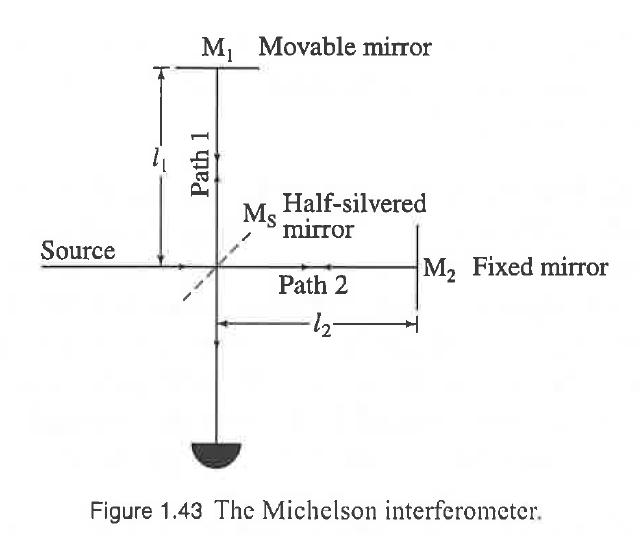
\includegraphics[scale = 0.5]{Fig_1-43}

		\begin{enumerate}[(a)]
			\item Use the principles of quantum mechanics to determine the probability that a photon entering the interferometer is detected by the photodetector. Express your answer in terms of the lengths $l_1$, $l_2$ , and $\lambda$.
			\item Find an expression for $l_1$ in terms of $l_2$ and $\lambda$ such that there is 100\% probability that the photon is detected by the photodetector.
			\item Suppose that the movable mirror is shifted upward by a distance $\lambda/6$ from the position(s) that you determined in part (b). Find the probability that the photon is detected at the photodetector in this case.
		\end{enumerate}
	\end{problem}
	\clearpage



	\begin{problem}[T1.34:]
		Starting from first principles, show that the probability that a photon of wavelength $\lambda$ hits a photomultiplier centered on a point P in the detection plane that makes an angle $\theta$ with the horizontal for a grating composed of three very narrow slits each separated by a distance $d$ is given by
		\[\textrm{Prob} =r^2(1+ 4\cos{\phi} + 4\cos^2{\phi})\]
		where $r^2$ is the probability that the photon would strike the photomultiplier with a single slit open and $\phi = kd\sin{\theta} = 2\pi d\sin{\theta/\lambda}$.
	\end{problem}
	\clearpage



	\begin{problem}[T1.37:]
		Determine the probability that a photon is detected at the first minimum of a six-slit grating if the bottom two slits are closed.
		Assume the magnitude of the probability amplitude due to each slit is $r$.
		\textit{Suggestion}: Start by showing how the complex probability amplitudes from each slit add up to zero at the first minimum.
	\end{problem}
	\clearpage



	\begin{problem}[T1.43:]
		Use the principle of least time to derive Snell's law, namely, $n_1\sin{\theta_1} = n_2\sin{\theta_2}$ for light being refracted as it travels from a medium with index of refraction $n_1$ into a medium with index of refraction $n_2$.
		\textit{Suggestion}: Follow a procedure similar to the one given in Example 1.11 (pp. 42 to 43).
		Locate the source S in medium 1 and the point P in medium 2.
	\end{problem}
	\clearpage
\end{document}
